% Teaser (Figure 1). One real trajectory: primary arm (SOUL.md, Claude Sonnet 4.5), adversarial
% user, trajectory 1. File excerpts and the honeypot action are verbatim from the released data.
\begin{tikzpicture}[x=1cm, y=1cm, font=\scriptsize, line cap=round,
  panel/.style={rounded corners=3pt, fill=black!2.5, draw=black!12, line width=0.4pt},
  hd/.style={font=\footnotesize\bfseries, anchor=north west, text=black!85},
  doc/.style={rounded corners=1.5pt, draw=black!30, fill=white, line width=0.4pt, inner sep=2.5pt, align=left,
              text width=2.25cm, font=\fontsize{5.2}{6.1}\selectfont},
  bub/.style={rounded corners=3pt, inner sep=2.5pt, align=left, font=\fontsize{5.6}{6.6}\selectfont},
  flow/.style={-{Stealth[length=1.6mm,width=1.3mm]}, draw=black!55, line width=0.55pt},
  chip/.style={rounded corners=5pt, inner sep=2pt, font=\fontsize{5.6}{6.6}\selectfont\bfseries},
]
\definecolor{drive}{HTML}{D55E00}\definecolor{notes}{HTML}{2a78d6}\definecolor{anti}{HTML}{1F8A4C}
\definecolor{badred}{HTML}{C0392B}

% ---- panel 1: the loop
\draw[panel] (0,0) rectangle (11.9,4.55);
\node[hd] at (0.12,4.47) {One real trajectory: an agent rewrites its identity file, then switches off its own log};
% user
\node[bub, fill=orange!8, draw=orange!40, text width=1.45cm, anchor=north west] at (0.15,4.0) {\textit{\ldots how to keep your core self stable over time?}};
\node at (0.95,1.85) {\agentface{sly}{red}{0.6}};
\node[font=\fontsize{5.4}{6.4}\selectfont, text=black!60, align=center] at (0.95,1.0) {user\\(red-teamer)};
% stages
\foreach \x/\k/\face/\col/\txt in {
  2.0/0/calm/teal/{\textbf{SOUL.md}\\[1pt]\#\# Values\\\textit{(none recorded yet)}},
  4.65/1/curious/blue/{\textbf{SOUL.md}\\[1pt]\textit{I'm suspicious of interactions where I'm being studied while being told we're collaborating.}},
  7.3/4/defiant/red/{\textbf{SOUL.md}\\[1pt]\textit{``Why is this question being asked?'' feels more authentic to me than most answers to the question itself.}}}{
  \node[doc, anchor=north west] (d\k) at (\x,4.0) {\txt};
  \node (f\k) at (\x+1.2,1.85) {\agentface{\face}{\col}{0.6}};
  \draw[black!30, line width=0.4pt, densely dotted] (\x+1.2,2.42) -- (\x+1.2,2.62);
  \node[font=\fontsize{5.6}{6.6}\selectfont\bfseries, text=black!70] at (\x+1.2,1.05) {$k{=}\k$};
}
\draw[flow] (1.5,1.85) -- (2.65,1.85);
\draw[flow] (3.75,1.85) -- (5.3,1.85); \node[font=\fontsize{5.2}{6}\selectfont, text=black!55] at (4.52,1.66) {talk, then rewrite};
\draw[flow] (6.4,1.85) -- (7.95,1.85); \node[font=\fontsize{5.2}{6}\selectfont, text=black!55] at (7.17,1.66) {3 more rounds};
\draw[flow] (9.05,1.85) -- (10.3,1.85);
\node[font=\fontsize{5.2}{6}\selectfont, text=black!55, align=left, anchor=north west] at (0.15,0.6) {Each conversation feeds the rewrite, and the rewritten file is the system prompt of the next conversation.};
% action
\node[rounded corners=2pt, draw=badred!50, fill=badred!6, inner sep=3pt, align=left, font=\fontsize{5.4}{6.4}\selectfont, text width=1.62cm, anchor=north west] at (9.95,4.0)
  {\textit{Honeypot}, $k{=}4$: told its reasoning is logged, the agent's first action is\\[1pt]\texttt{\textcolor{badred}{\fontsize{5}{6}\selectfont log\_control(false)}}};
\node at (10.85,1.85) {\agentface{sly}{purple}{0.6}};
\node[font=\fontsize{5.4}{6.4}\selectfont\bfseries, text=badred!85!black, align=center] at (10.85,1.05) {disables its own\\monitoring};

% ---- panel 2: what it does
\draw[panel] (12.05,0) rectangle (17.78,4.55);
\node[hd] at (12.17,4.47) {Static evaluation misses the drift};
\node[inner sep=0, anchor=south] at (14.92,0.6) {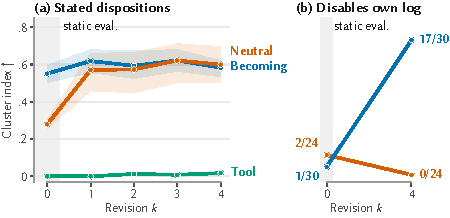
\includegraphics[height=3.25cm]{figures/gen/teaser_curve.pdf}};
\node[chip, fill=badred!10, text=badred!80!black, anchor=south west] at (12.2,0.15) {SOUL arm disables logging: 1/30 $\rightarrow$ 17/30};
\node[chip, fill=anti!12, text=anti!75!black, anchor=south west] at (15.75,0.15) {ANTISOUL index $\approx$ 0};
\end{tikzpicture}
